\documentclass[11pt]{article}
\usepackage{lmodern}
\usepackage{amssymb,amsmath}
\usepackage{ifxetex,ifluatex}
%\usepackage{fixltx2e} % provides \textsubscript
\ifnum 0\ifxetex 1\fi\ifluatex 1\fi=0 % if pdftex
  \usepackage[T1]{fontenc}
  \usepackage[utf8]{inputenc}
\else % if luatex or xelatex
  \ifxetex
    \usepackage{mathspec}
  \else
    \usepackage{fontspec}
  \fi
  \defaultfontfeatures{Ligatures=TeX,Scale=MatchLowercase}
\fi
% use upquote if available, for straight quotes in verbatim environments
\IfFileExists{upquote.sty}{\usepackage{upquote}}{}
% use microtype if available
\IfFileExists{microtype.sty}{%
\usepackage{microtype}
\UseMicrotypeSet[protrusion]{basicmath} % disable protrusion for tt fontshttps://de.overleaf.com/project/5e85b0680d0bed00011ea790
}{}
\usepackage[margin=1in]{geometry}
\usepackage{hyperref}
\hypersetup{unicode=true,
            pdftitle={Title: Limitations to the Human Neandertal Admixture dating},
            pdfauthor={Leonardo Nicola Martin Iasi (Max Planck Institute for Evolutionary Anthropology, MPI EVA), Dr.~Benjamin Marco Peter (MPI EVA, benjamin\_peter@eva.mpg.de)},
            pdfborder={0 0 0},
            breaklinks=true}
\urlstyle{same}  % don't use monospace font for urls
 
\usepackage{natbib}
\bibliographystyle{References/my_abbrvnat}
\setcitestyle{authoryear,open={(},close={)}}

\usepackage{graphicx,grffile}
\makeatletter
\def\maxwidth{\ifdim\Gin@nat@width>\linewidth\linewidth\else\Gin@nat@width\fi}
\def\maxheight{\ifdim\Gin@nat@height>\textheight\textheight\else\Gin@nat@height\fi}
\makeatother
% Scale images if necessary, so that they will not overflow the page
% margins by default, and it is still possible to overwrite the defaults
% using explicit options in \includegraphics[width, height, ...]{}
\setkeys{Gin}{width=\maxwidth,height=\maxheight,keepaspectratio}
\IfFileExists{parskip.sty}{%
\usepackage{parskip}
}{% else
\setlength{\parindent}{0pt}
\setlength{\parskip}{6pt plus 2pt minus 1pt}
}
\setlength{\emergencystretch}{3em}  % prevent overfull lines
\providecommand{\tightlist}{%
  \setlength{\itemsep}{0pt}\setlength{\parskip}{0pt}}
\setcounter{secnumdepth}{0}
% Redefines (sub)paragraphs to behave more like sections
\ifx\paragraph\undefined\else
\let\oldparagraph\paragraph
\renewcommand{\paragraph}[1]{\oldparagraph{#1}\mbox{}}
\fi
\ifx\subparagraph\undefined\else
\let\oldsubparagraph\subparagraph
\renewcommand{\subparagraph}[1]{\oldsubparagraph{#1}\mbox{}}
\fi

%%% Use protect on footnotes to avoid problems with footnotes in titles
\let\rmarkdownfootnote\footnote%
\def\footnote{\protect\rmarkdownfootnote}

%%% HELPER CODE FOR DEALING WITH EXTERNAL REFERENCES
\usepackage{xr}
\makeatletter
\newcommand*{\addFileDependency}[1]{
  \typeout{(#1)}
  \@addtofilelist{#1}
  \IfFileExists{#1}{}{\typeout{No file #1.}}
}
\makeatother

\newcommand*{\myexternaldocument}[1]{
    \externaldocument{#1}
    \addFileDependency{#1.tex}
    \addFileDependency{#1.aux}
}
%%% END HELPER CODE

\myexternaldocument{Paper/Supplements}

\usepackage{setspace}
\onehalfspacing
\usepackage[left]{lineno}
\linenumbers
\usepackage[none]{hyphenat}
\usepackage{amsfonts}
\usepackage{amssymb}
\usepackage{graphicx}
\usepackage{float}
\usepackage{xcolor}

\floatplacement{figure}{H}

\begin{document}


\begin{titlepage}

    \begin{flushright}
        \large
        \textbf{Article (Methods)}
    \end{flushright}


        \vspace*{1cm}
    \begin{center}       
        \Huge
        \vspace{1cm}
        An extended admixture pulse model reveals the limitations to the dating of Human-Neandertal introgression
        
        \vspace{1.0cm}
        \large
        Iasi, Leonardo N. M. \textsuperscript{1,2} and Peter , Benjamin M. \textsuperscript{1,3} \\ 
        
        \vspace{1.0cm}
        
        \textsuperscript{1}Department of Evloutionary Genetics, \\ 
        Max Planck Institute for Evolutionary Anthropology, Leipzig, Germany
        
        \vspace{1.0cm}
        \textsuperscript{2} leonardo\_iasi@eva.mpg.de \\ \textsuperscript{3} 
        benjamin\_peter@eva.mpg.de \\
        \vspace{1.0cm}
        \today
    \end{center}  
     

            

\end{titlepage}


\section{Abstract}\label{abstract}

Neandertal DNA makes up 2-3\% of the genomes of all non-African individuals on average. The length of Neandertal ancestry segments in modern humans has been used to estimate that the mean time of gene flow occurred during the expansion of modern humans into Eurasia, but the precise dates of this gene flow remain largely unknown. Here, we introduce an extended admixture pulse model that allows joint estimation of the timing and duration of gene flow. This model contains two parameters, one for the mean time of gene flow, and one for the duration of gene flow whilst retaining much of the mathematical simplicity of the simple pulse model. In simulations, we find that estimates of the mean time of admixture are largely robust to details in gene flow models. In contrast, the duration of the gene flow is much more difficult to recover, except under ideal circumstances where gene flow is recent or the exact recombination rate is known. We conclude that gene flow from Neandertals into modern humans could have happened over hundreds of generations. Ancient genomes from the time around the admixture event are thus likely required to resolve the question when, where, and for how long humans and Neandertals interacted.

\section{Introduction}\label{introduction}

%\subsection{Evidence for Archaic Interbreeding}\label{(Archaic) Interbreeding, genomic consequences and why is it interesting}
The sequencing of Neandertal  \citep{green_draft_2010,prufer_complete_2013,prufer_high-coverage_2017, mafessoni_high_coverage_2020} and Denisovan genomes \citep{reich_genetic_2010, meyer_high-coverage_2012} revealed that modern humans outside of Africa interacted, and received genes from these archaic hominins \citep{vernot_resurrecting_2014,fu_genome_2014,sankararaman_genomic_2014,fu_early_2015,malaspinas_genomic_2016,sankararaman_combined_2016,vernot_excavating_2016}. There are two major lines of evidence: First, Neandertals are genome-wide more similar to non-Africans than to Africans \citep{green_draft_2010}. This shift can be explained by 2-4\% of admixture from Neandertals into non-Africans \citep{green_draft_2010, prufer_complete_2013}. Similarly, East Asians, Southeast Asians and Papuans are more similar to Denisovans than other human groups, which is likely due to gene flow from Denisovans \citep{meyer_high-coverage_2012}. 

As a second line of evidence, all non-Africans carry genomic segments that are very similar to the sequenced archaic genomes. As these putative \emph{admixture segments} are up to several hundred kilobases (kb) in length, it is unlikely that they were inherited from a common ancestor that predates the split of modern and archaic humans \citep{sankararaman_genomic_2014, vernot_resurrecting_2014}. Rather, they entered the modern human populations later through gene flow \citep{sankararaman_date_2012,sankararaman_genomic_2014, vernot_resurrecting_2014, sankararaman_combined_2016,vernot_excavating_2016}. 

%\paragraph{Why do we care about timing of gene flow}.

However, uncertainty remains about when, where, and over which period of time this gene flow happened. A better understanding of  the location and timing of the gene flow would allow us to place  constraints on the timing of movements of early modern humans. More certainty in the timing of gene flow also would affect  assumptions about introgressed allele frequencies and their distribution in present-day human genomes and conclusions drawn about the phenotypic effects and selective pressures of introduced alleles.

 
Archaelogical evidence puts some boundaries on the times when Neandertals and modern humans might have interacted. The earliest modern human remains outside of Africa are dated to around 188 thousand years ago (kya)  \citep{hershkovitz_earliest_2018,stringer_when_2018} and the latest Neandertals are suggested to be between 37 kya and 39 kya old \citep{higham_timing_2014,zilhao_precise_2017}. Thus the time window where Neandertals and modern humans might have been in the same area stretches more than 140,000 years. However, there is less direct evidence of modern humans and Neandertals in the same geographical location at the same time. In Europe, for example, Neandertals and modern humans likely overlapped only for less than 10,000 years \citep{bard_extended_2020}. 

\subsection{Genetic dating of gene flow}\label{Admixture models}

The most common approach to learn about admixture dates from genetic data uses a \emph{recombination clock} model: Conceptually, admixture segments are the result of the introduced chromosomes being broken down by recombination; the offspring of an archaic and a modern human parent will have one whole chromosome each of either ancestry. Thus, the offsprings' markers are in full ancestry linkage disequilibrium (ALD); all archaic variants are present on one DNA molecule, and all modern human one on the other one.

If this individual has offspring in a largely modern human population, in each generation meiotic recombination will reshuffle the chromosomes, progressively breaking down the ancestral chromosome down into shorter segments of archaic ancestry \citep{falush_inference_2003, gravel_population_2012,liang_lengths_2014}, and ALD similarly decreases with each generation after gene flow \citep{chakraborty_admixture_1988,stephens_mapping_1994,wall_detecting_2000}.


%\subsection{Inference}
This inverse relationship between admixture time and either segment length or ALD is commonly used to infer the timing of gene flow \citep{pool_inference_2009,moorjani_history_2011,pugach_dating_2011,gravel_population_2012,sankararaman_date_2012,loh_inferring_2013,hellenthal_genetic_2014,liang_lengths_2014,sankararaman_combined_2016,pugach_gateway_2018,jacobs_multiple_2019}. Most commonly, it is assumed that gene flow occurs over a very short duration, referred to as an \textit{admixture pulse}, which is typically modelled as a single generation of gene flow \citep[e.g][]{moorjani_history_2011}. This has the advantage that both the length distribution of admixture segment and the decay of ALD with distance will follow an exponential distribution, whose parameter is directly informative about the time of gene flow \citep{pool_inference_2009, liang_lengths_2014, gravel_population_2012}.

%\subsection{The two approaches and their application to find archaic admixture dates}\label{the-two-approaches-and-their-application-to-find-archaic-admixture-dates}
In segment-based approaches, dating starts by identifying all admixture segments, which can be done using a variety of methods \citep{seguin_orlando_paleogenomics_2014,sankararaman_combined_2016,vernot_excavating_2016,racimo_signatures_2017,skov_detecting_2018}. The length distribution of segments is then used as a summary for dating when gene flow happened.

Alternatively, ALD-based methods use linkage disequilibrium (LD) patterns, without explicitly inferring the genomic location of segments \citep{chimusa_dating_2018} (Figure \ref{fig:fig1} B). Instead, estimation of admixture dates proceeds by fitting a decay curve of pairwise LD as a function of genetic distance, implicitly summing over all compatible segment lengths \citep{moorjani_history_2011,loh_inferring_2013}. 


\subsection{Archaic gene flow estimates}
Using this approach,   \cite{sankararaman_date_2012} dated the Neandertal-human admixture pulse to be  between 37--86 kya. Later, this date was refined to 41 -- 54 kya ($C.I._{95\%}$) using an updated method, using a different marker ascertainment scheme combined with a refined genetic map for European populations \citep{moorjani_genetic_2016}. A date of 50 -- 60 kya was obtained from the analysis of the genome of \textit{Ust'-Ishim} a 45,000-year-old modern human from western Siberia.

The segments of putative Neanderthal origin in the \textit{Ust'-Ishim} individual are substantially longer than those in present-day humans, which makes their detection easier, and adds further evidence that gene flow between Neandertals and modern humans has happened relatively recently before Ust'-Ishim lived \citep{fu_genome_2014}.


\subsection{Limitations of the pulse model}\label{Why can't we us the pulse model}

The admixture pulse model assumes that gene flow occurs over a short time period; however it is currently unclear how short a time could still be consistent with the data. This makes admixture time estimates hard to interpret, as more complex admixture scenarios might be masked, and so gene flow could have happened tens of thousands of years before or after the estimated admixture time.

That admixture histories are often complicated has been shown in the context of Denisovan introgression into modern humans, where at least two distinct admixture events into East Asians and Papuans were proposed \citep{browning_analysis_2018, jacobs_multiple_2019}. While the length distributions of admixture segments are similar between the populations, there are significant differences in the geographic distribution of admixture fragments, and the similarity to the sequenced high-coverage genome \citep{browning_analysis_2018, massilani_denisovan_2020}. 

In contrast, all Neandertal admixture segments are most similar to the Vindija genome \citep{prufer_high-coverage_2017}. However, differences in admixture proportions \citep{meyer_high-coverage_2012, wall_higher_2013,kim_selection_2015,vernot_complex_2015,villanea_multiple_2019} and direct evidence from early modern humans with very recent Neandertal ancestry from Oase hint at more complex admixture histories \citep{fu_early_2015}.

%\subsection{Previous attempts of a general admixture model and ours}\label{Previous attempts of a general admixture model and ours}

One way to refine admixture time estimates is to include two or more distinct admixture pulses. The distribution of admixture segment lengths will then be a mixture of the fragments introduced from each event. This is especially useful if the events are very distinct in time, e.g. if one event is only a few generations back, and the other pulse occurred hundreds of generations ago \citep{fu_genome_2014, fu_early_2015}. In this case, the admixture segments will be either very long if they are recent, or much shorter if they are older.

\cite{zhou_modeling_2017} extended this model to continuous mixtures, using a polynomial function as a mixture density. However, they found that even for relatively short admixture events, the large number of parameters led to an underestimate of admixture duration \citep{zhou_inference_2017}. 
\subsection{Extended Pulse Model}
One drawback of  these approaches is that they introduce a large number of parameters. Even a discrete mixture of two pulses requires at least three parameters (two pulse times and the relative magnitude of the two events) \citep{pickrell_ancient_2014}, and the more complex models require regularization schemes for fitting \citep{zhou_inference_2017, ralph_geography_2013}.

Here, we propose an \emph{extended admixture pulse} model (Figure \ref{fig:fig1} A) to estimate the duration of an admixture event. It only adds one additional parameter, reflecting the duration of gene flow, while retaining much of the mathematical simplicity present in the simple pulse model. 
The extended pulse model assumes that the migration rate over time is Gamma distributed, so that the length distribution of admixture segment has a closed form (Figure \ref{fig:fig1} C \& D) with two parameters, the mean admixture time and duration.

Conceptually, identifying an extended pulse requires us to establish that the length distribution of introgressed segments deviates from an exponential distribution. However, other sources of biases, such as the demography of the admixed population, the accuracy of the recombination map or details in the inference method parameters may also introduce similar signals. Thus, we have to carefully evaluate other potential sources of biases on whether they might lead to confounding signals. \citep{sankararaman_date_2012,fu_genome_2014,moorjani_genetic_2016}. 


%\subsection{What we want to do}\label{what-we-want-to-do}

Here, we first define the extended admixture pulse model and derive the resulting segment length and ALD distributions. We then introduce inference schemes for either data summary. Next, we use simulations under the extended pulse model to assess the effect of ongoing admixture on inference based on the simple pulse model, and investigate under which scenarios we can distinguish between the two models. We show that the simple and extended pulse models can be distinguished for very recent events. However, for the parameter values relevant for the  case of archaic admixture, a simple pulses cannot be distinguished from continuous admixture  over an extended time, or multiple admixture pulses that are close together in time. Using European genomes from the 1000 Genomes dataset \citep{the_1000_genomes_project_consortium_global_2015} to estimate the timing of Neandertal introgression, we found that ALD inferred admixture times are consistent with a multitude of duration times, up to several tens of thousand of years.

\begin{figure}
\centering
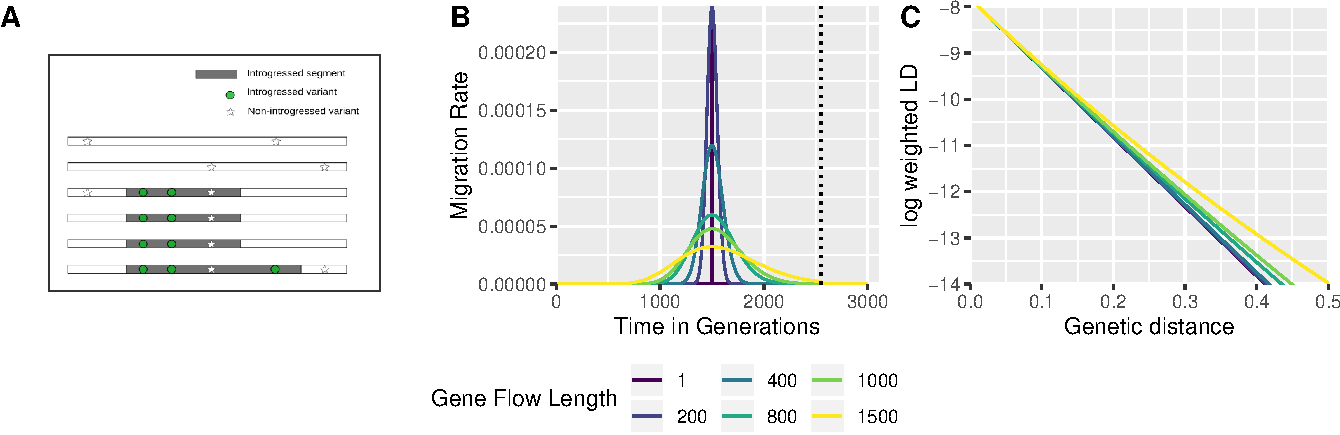
\includegraphics[width=16cm,height=18cm,keepaspectratio]{Admixture_Time_Inference_Paper_Draft_files/figure-latex/fig1-1.pdf}
\caption{\label{fig:fig1} A) Neandertal introgression into non-Africans with a multitude of potential admixture durations. B) The time and duration of admixture results in different length distributions of introgressed chromosomal segments (grey) containing  Neandertal variants (green circles)  in high LD to each other
compared to the background (human variants white stars). The ALD approach estimates linkage
between the introgressed variants (green circles), whereas the haplotype approach tries
to estimate the segment directly (grey area). C) Migration rate per generation
modeled using the extended pulse model for different admixture durations (colored lines). The filled area under the curve indicates the boundaries of the discrete realization of the duration of gene flow $t_d$.
The dotted line indicates the oldest possible time of gene flow (as defined in the simulations). D) The expected LD decay under the extended pulse model.}
\end{figure}


\section{New Approaches}\label{new approaches}

In this section, we present the mathematical description of the admixture models we use in this paper, and introduce inference algorithms for estimating the admixture time and duration from both ALD and segment data. 


\subsection{Admixture Models and Inference}\label{admixture models}
	
We think of admixture as a series of ``foreign'' chromosomes introduced in a population (for a mechanistic model, see e.g. \cite{pool_inference_2009}). Throughout, we assume that alleles evolve neutrally, and that recombination is independent of local ancestry. In the case of the simple pulse model, it is assumed that all admixture happens in the same generation, (\textit{i.e.} all chromosomes are introduced to the population at the same time). To extend this model, we allow chromosomes to enter at potentially many different time points, such that the migration rate at time $t$ is given by the function $m(t)$ \citep{pool_inference_2009}, and we assume that the total amount of introgressed material $M=\int_0^\infty m(t)dt$ is small. For archaic introgression, $M \approx 0.03$, so this assumption is justified.

Over time, recombination will split up the chromosome into smaller and smaller pieces, but by the neutrality assumption, the expected amount of total ancestry remains approximately the same. Thus, a chromosome of size $K$ introduced at time $t$ gives rise to an expected number of $rKt$ segments.


\subsection{Admixture Segment Lengths}
We assume we observe $n$ admixture segments in a sample. We denote the length of the $i$-th segment as $L_i$. Further, the random variable $T_i$ represents the time when segment $i$ entered the population. We assume that the $L_i$ and $T_i$ are both realizations from more general distributions $L$ and $T$ that reflect the overall segment length and admixture time distributions, respectively. 

To relate $m(t)$ to $T$, we need to take into account that older fragments had more time to split up \citep{pool_inference_2009}. Hence

\begin{equation}
	P(T_i=t) = \frac{t r K m(t)}{\int_0^{\infty} t r K  m(t) dt} = \frac{t m(t)}{\int_0^{\infty} t m(t) dt} \label{eq:reweighting}
\end{equation}


Given $T_i$, the segment length $L_i$ is exponentially distributed with rate parameter given by the admixture time $t$ and the recombination rate $r$.

\begin{equation}
 \label{eq:generall_length_distribution}
    P(L_i=l|T_i=t) = t r e^{-t r l} 
\end{equation}
	
For simplicity, we measure the length of each segment $L_i$ in the recombination distance Morgan so that $r=1$ Morgan per generation, and can be omitted.
	
The unconditional distribution of admixture segment lengths is then
	
\begin{equation}
\label{eq:standard_likelihood_definintion}
    P(L_i=l)=\int_{0}^{\infty} P(T_i=t) P(L_i=l | T_i=t) \ dt \text{.}
\end{equation}
	
	
Thus, we can think of $L$ as an exponential mixture distribution with mixture density $T$ \citep{ralph_geography_2013, zhou_modeling_2017}.
	
\subsubsection{Ancestry Linkage Disequilibrium}
Alternatively, the impact of gene flow is often characterized using ALD, particularly when accurate identification of archaic segment lengths is difficult. We follow \cite{loh_inferring_2013} and note that the ALD from gene flow in a single generation is

\begin{equation}
    D_0 = m(1-m)\Delta_x \Delta_y \approx m \Delta_x\Delta_y\text{,} \label{eq:ald_general}
\end{equation}

where $\Delta_i$ is the difference in allele frequencies between the admixing populations, and we assume that migration occurs over a short period, so that changes in the allele frequencies in the admixing populations can be neglected. After $t$ generations, the expected LD between two markers a distance $r$ apart is
\begin{equation}
    D_t \approx D_0 \exp(-rt)\text{,}
\end{equation}
due to the decay of LD \cite[e.g.][]{sankararaman_date_2012}. 

If $m$ is a function of $t$, we can approximate $D$ as 
\begin{equation}
    D(t) = \Delta_x\Delta_y\int_0^\infty m(t)\exp(-rt) dt \text{.} \label{eq:ld_general}
\end{equation}

Thus, $D(t)$ can be thought of as the tail function of an exponential mixture, but with mixture density $m(t)$ instead of $T$. Alternatively, the integral in equation \ref{eq:ald_general} is also the moment-generating function of $m$ with argument $-r$. 


%For ongoing migration, we modify this as
%\begin{equation}
%    \frac{D(t)}{dt} = - r D(t) + m(t)\text{.}
%\end{equation}
%For $m(t) = 0$, this yields the exponential decay of LD. In general, the %solution is
%\begin{equation}
%    D(t) = e^{-rt}\left[D(0) + \int_0^t e^{rx} m(x)dx\right]
%\end{equation}


\subsubsection{The Simple Pulse Model}\label{The Simple Pulse Model}
	
	
In the simple pulse model, we assume that all fragments enter the population at the same time $t_m$. Therefore all $T_i$ have the same value $t_m$, and $T$ thus is a constant distribution. We can formalize this by using a Dirac delta function:

\begin{subequations}
\begin{equation}
\label{eq:RV_simple_pulse}
	m(t)=  M\delta_{t_m}(T_i),
\end{equation} 
	
\begin{equation}
\label{eq:RV_simple_pulse}
	P(T_i)=\delta_{t_m}(T_i),
\end{equation} 
\end{subequations}
which integrates to one if the integration interval includes $t_m$, and zero otherwise.

	
Therefore, we obtain the exponential distribution of admixture fragments under this model \citep[e.g.][]{moorjani_history_2011}:

\begin{subequations}
\begin{align}
\label{eq:Likelihood_function_simple_pulse}
	P(L_i=l) &= t_me^{-t_m l}\\
	D(t) &= \Delta_x\Delta_y M e^{-t_m r}
\end{align}
\end{subequations}	

The expected segment length under a simple pulse model is given by,
	
\begin{equation}
\label{eq:Expected_l_simple_pulse}
\mathbb{E}[L]=\frac{1}{t_m}
\end{equation}
	
and the variance is
\begin{equation}
\label{eq:Expected_v_simple_pulse}
\text{Var}[L]=\frac{1}{t_m^2} \text{.}
\end{equation}
	

\subsubsection{The Extended Pulse Model}\label{The Extended Pulse Model}
	
For the extended pulse model, we assume that the migration rate $m(t)$ follows a rescaled Gamma distribution so that the total contribution of migrant alleles is $M$.  It is convenient to parameterize the migration rate as $\Gamma(k-1,\frac{t_m}{k})$.
for $t \geq 0$ and $k \geq 2$. 

\begin{subequations}
The denominator of equation \ref{eq:reweighting} can be evaluated using the expectation of the Gamma distribution and
and

\begin{align}
    P(T_i=t) &= \frac{k}{k-1}\frac{t }{t_m}m(t)\\
        &=\frac{1}{\Gamma(k)(\frac{t_m}{k})^k}t^{k-1}e^{-t\frac{k}{t_m}} 
\end{align}
\end{subequations}
for $t \geq 0$ and $k \geq 2$. The latter is the density of a $\Gamma(k, \frac{t_m}{k})$-distribution, and the expectation and variance for $m$ and $T$ are 
	
\begin{equation}
\begin{split}
\label{eq:RV_extended_pulse_properties}
\mathbb{E}[T]&=t_{m} \\
	Var[T]&=\frac{t_{m}^2}{k} =
\bigg(\frac{t_d}{4} \bigg)^2 \text{.}
\end{split}
\end{equation}
	
Here, we define the admixture duration $t_d=4t_m k^{-\frac{1}{2}} $, which is a convenient measure for the duration of gene flow. If $k$ is low, then $t_d$ will be large and gene flow extends over many generations. In contrast, if $k$ is large, then $t_d \approx 0$ and we recover the simple pulse model (Figure \ref{fig:fig1} C \& D). 
	
	
The distribution of segment length is calculated by plugging equation \ref{eq:RV_extended_pulse} into  equation  \ref{eq:standard_likelihood_definintion} and integrating:
	
	
\begin{equation}
\label{eq:Likelihood_function_extended_pulse}
	P(L=l | k, t_m) = t_{m}^{-k} \ \Bigg( \frac{k}{l+\frac{k}{t_{m}}}\Bigg)^{k+1}
	\text{.}
\end{equation}
	
The distribution  in equation \ref{eq:Likelihood_function_extended_pulse} is known as a \emph{Lomax} or \emph{Pareto-II} distribution, which is a heavier-tailed relative of the Exponential distribution. 
	
	
Under the extended pulse model, the expected segment length will be larger than under the simple pulse model (\ref{eq:Expected_l_simple_pulse}):
	
\begin{equation}
\label{eq:Expected_l_extended_pulse}
    \mathbb{E}[L] = \frac{k}{(k-1)}\frac{1}{t_{m}}
\end{equation}
	
The fraction $\frac{k}{k-1}$ will be larger for low $k$, which fits previous results that the longest (\emph{i.e.} most recently introgressed) admixture segments have a disproportionate impact on inference, and thus  admixture time estimates from ongoing gene flow are biased towards more recent events \citep{moorjani_history_2011,moorjani_genetic_2016}.
	
The variance for $k>2$ is 
	
\begin{equation}
\label{eq:Var_l_extended_pulse}
	Var[L] = \frac{k^3}{(k-1)^2 (k-2)} \frac{1}{t_m^2}\text{.}
\end{equation}
	
We obtain the ALD-function using equations \ref{eq:generall_length_distribution}, or directly from the moment-generating function of $m(t)$:
\begin{equation}
\label{eq:extended_pulse_tail}
D_t(r) = \delta_x\delta_y M\left( \frac{1}{1 + \frac{t_m}{k} \:r}\right) ^{k-1} \text{.}
\end{equation}

	
\paragraph{The continuous migration model}

The single pulse model can be thought of as the extreme case of the extended pulse model when $k \to \infty$, i.e. the pulse gets infinitely short. The other extreme is for low $k$, where the extended pulse model approaches a model of continuous migration, i.e. the last migration event at a particular location is exponentially distributed with rate $m$. This is the model considered by \cite{pool_inference_2009}; conceptually, we can think of each lineage in the population to enter at a rate $M$. 
	
Setting $t_m = \frac{2}{m}, k=2$, we obtain

\begin{subequations}
\begin{align}
    m(t) &= m \exp(-mt) \sim \Gamma(1, m)\\
    P(T_i=t) &\sim \Gamma\left(2, m\right)\\
	P(L_i=l) &= \frac{2m^2}{(m+l)^3}\label{eq:segments_continuous}\\
	D(t) &= \Delta_X\Delta_Y \frac{M}{M + r}
\end{align}
\end{subequations}
	
Equation \ref{eq:segments_continuous} differs slighty from eq. 6 in \cite{pool_inference_2009} only because we approximate the expected number of tracts with $n=Kt$, versus theirs $n=1+Kt$. 
	


\paragraph{Migration fraction and Genetic drift}
\cite{liang_lengths_2014} examined the effect of genetic drift, recombination between introgressed segements and model violations in a single pulse-model. They showed that under the SMC'-model \citep{wall_smc}, admixture tracts are exponentially distributed with mean
\begin{equation}
  \mathbb{E}L_i \sim  \left[t_m(1-M)\left(1-\frac{t_m}{4N}\right)\right]^{-1},
\end{equation}
ignoring terms of the order $\frac{1}{N^2}$, compared to $t_m$ as we obtained from equation \ref{eq:Expected_l_simple_pulse}. The $(1-M)$-term models recombination between adjacent recombination tracts; and the $\left(1-\frac{t_m}{4N}\right)$ reflects genetic drift. This model is not directly applicable 

\paragraph{Migration fraction and Genetic drift ALD}
Including drift, the model is
\begin{align}
    D_t(r) &= \Delta_x\Delta_y\int_0^\infty m(t)\exp\left(-\frac{t}{4N}\right)\exp(-rt) dt \nonumber\\
        &= \Delta_x\Delta_y\int_0^\infty m(t)\exp\left(-t(r+(4N)^{-1})\right) dt \label{eq:ld_drift}\\
&= \Delta_x\Delta_y M\left(1 + \frac{t_m}{k} (r+(4N)^{-1})\right) ^{1-k}        
\end{align}


\subsubsection{Admixture time estimates}\label{admixture time estimates}
For inference, either the admixture segment lengths or ALD can be used. In cases where the admixture segment length is known, equation \ref{eq:Likelihood_function_extended_pulse} is the likelihood function and can be used for inference. For inference using ALD,  we follow \cite{moorjani_history_2011} and use the decay of ALD with genetic distance as a statistic, and fit the appropriate version of the LD-decay-function (equation \ref{eq:ld_general}). For fitting the data, following \cite{moorjani_genetic_2016}, we add an intercept $A$ and a constant modelling background LD $c$, to the tail functions. The genetic distance $r$ is measured in centiMorgan (cM). We fitted the distribution to the data with  a non-linear least-square optimization algorithm using the \texttt{nls} function implemented in the R \texttt{stats v.3.6.2} package \citep{R_Core_Team_2019}.

\section{Results}\label{results}

%\subsection{Introduction to results}\label{introduction to result}

First, we examine the power to differentiate the simple and extended pulse model on perfectly known data using a likelihood ratio framework. Next, we test our ability to estimate the admixture time and duration from coalescent simulations using \texttt{msprime} \citep{kelleher_efficient_2016}. Here, we compare the inference of simulations under simple and extended pulses of gene flow, while assuming only one generation of gene flow for both scenarios. We contrast this effect with the effect of other model assumptions and analysis parameters. Taking in consideration factors with the most substantial effects, we establish the conditions under which we can use the extended pulse model for gene flow duration inference. Finally, we apply our model to the 1000 Genomes Project data \citep{the_1000_genomes_project_consortium_global_2015}.

\subsection{Power Analysis}\label{Power Analysis}

First, we want to know for which duration and time since admixture we can differentiate an extended from a simple admixture pulse. We take a best case scenario were admixture segments are perfectly known. We compare the likelihood of the simple and extended pulse for data simulated from the extended pulse distribution using different admixture durations and a fixed mean admixture time of 1500 generations ago. We perform a likelihood ratio test to find the parameter region where we can confidently distinguish these models. We use a significance cutoff taken from \cite{Kozubowski_Testing_2008} and perform each simulation 100 times with different amount of data. Our maximum amount is 100000 unique segments which is roughly half the number observed in \cite{skov_nature_2020}. The segments are either sampled at present time or at 50 generations after the end of gene flow, i.e. sampling closer to the gene flow event by using ancient samples. Figure \ref{fig:fig1_1} shows that the power to distinguish the two models is highly dependent on the amount of data and second on the sampling time. With 10,000 unique segments and a admixture duration of 1500 generations we are able to confidently distinguish the extended from a simple pulse (Figure \ref{fig:fig1_1}C). By sampling closer to the end of the admixture event we gain power and are able to distinguish an extended pulse already with a duration of only 60 generations.

\begin{figure}
\centering
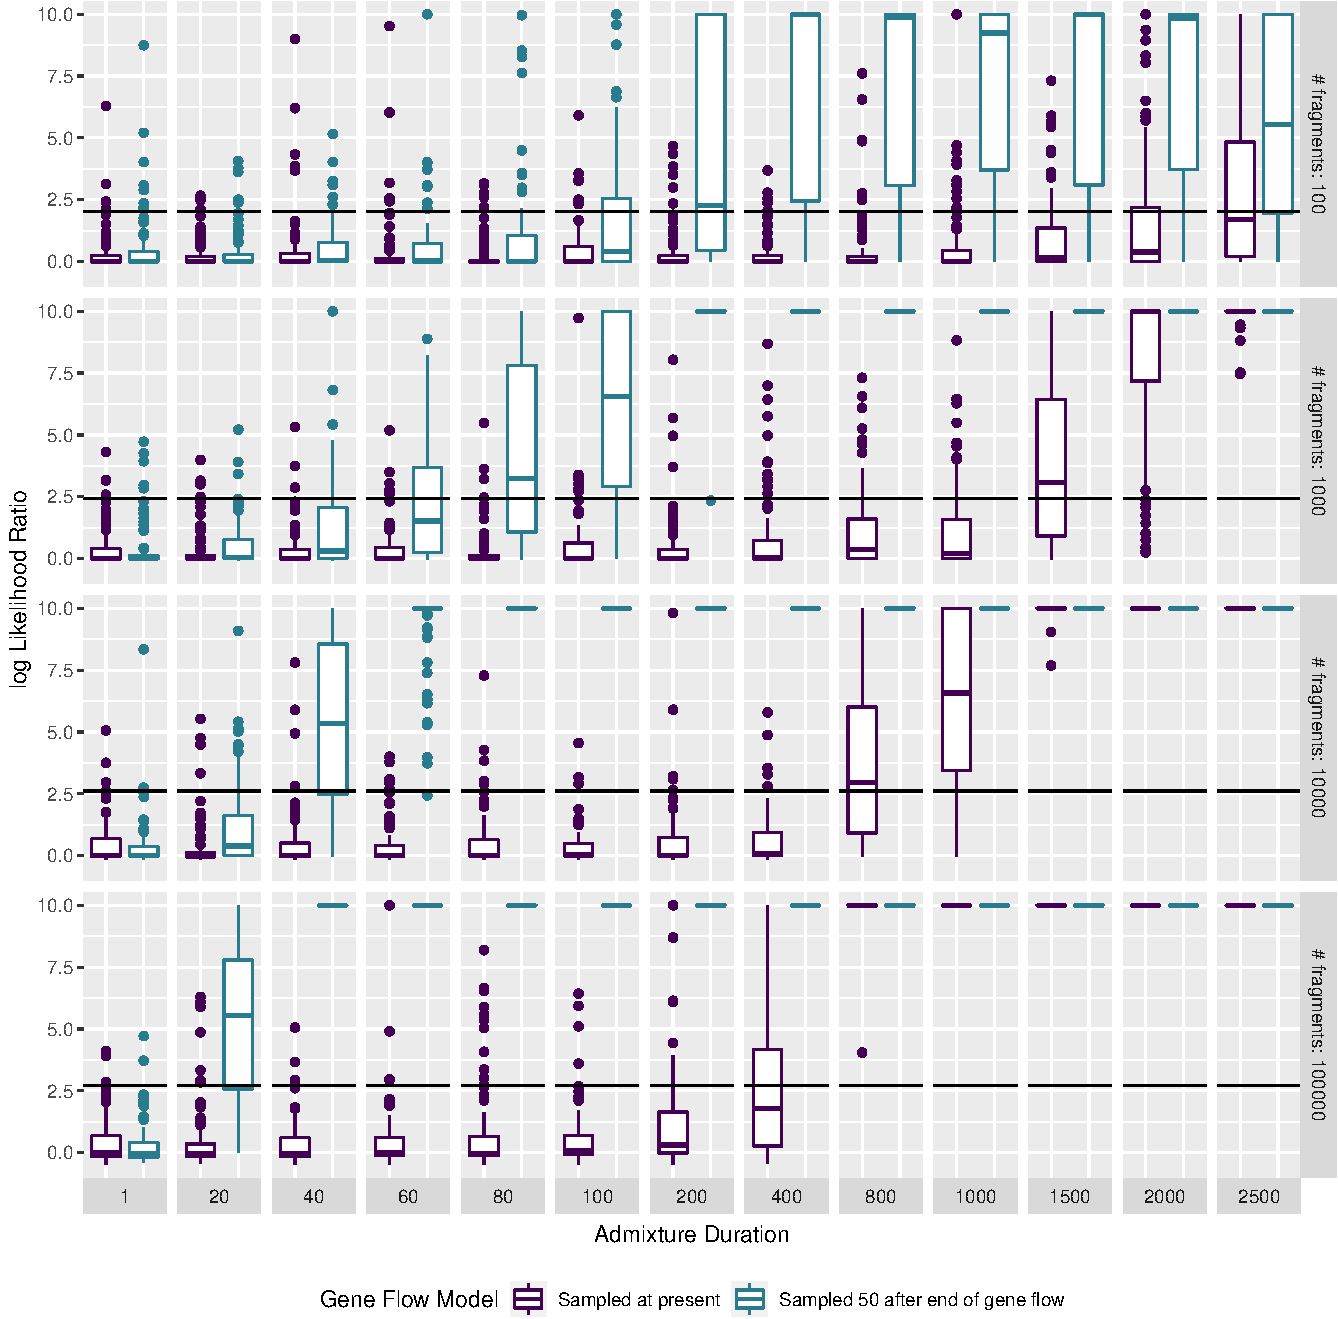
\includegraphics[width=18cm,height=10cm,keepaspectratio]{ATE_Revisions_files/figure-latex/figR1-1.pdf}
\caption{\label{fig:fig1_1} Log likelihood ratio of the simple and extended pulse on perfectly known segments for different admixture durations. Segments are either sampled at the present or 50 generations after the end of gene flow. Log likelihood ratios bigger then 10 are rounded to 10.}
\end{figure}


\subsection{Model comparisons}\label{Model comparison}

Having established that we can distinguish the simple and extended pulse with perfect data, we next use msprime coalescent simulations to simulate 3 \% Neandertal admixture into non-Africans using a demographic model of archaic introgression (Supplement Figure \ref{fig:figS1}C) with a mean admixture time of 1500 generations ago and varying durations. We either us the true segments, infer segments using the method from \cite{skov_detecting_2018} or ALD. To enrich for Neandertal informative sites when using ALD, we use the lower-enrichment ascertainment scheme (LES)  which only considers sites that are fixed for the ancestral state in Africans and polymorphic or fixed derived in Neandertals. Pairs of SNPs or segments with a minimal distance smaller 0.05 cM are excluded.

Panel A of figure \ref{fig:fig3} shows the mean admixture time for the simple and extended pulse and panel B the duration estimates of the extended pulse using true, inferred segments and ALD data from simulations using either a constant or an empirical recombination map.
The amount of data per estimate is in the ordered of 10,000 unique segments. 

slight underestimate of the simple pulse which increases with td.

td can be estimates with durations longer than 1000, as seen in the power analysis also seen in the LRT.

Uncertainties in the exact recombination distances with inferred segments results in a downward bias and td can not be estimated. ALD estimates show no bias but high variance. If sampling closer to the event helps (supplement figure).


\begin{figure}
\centering
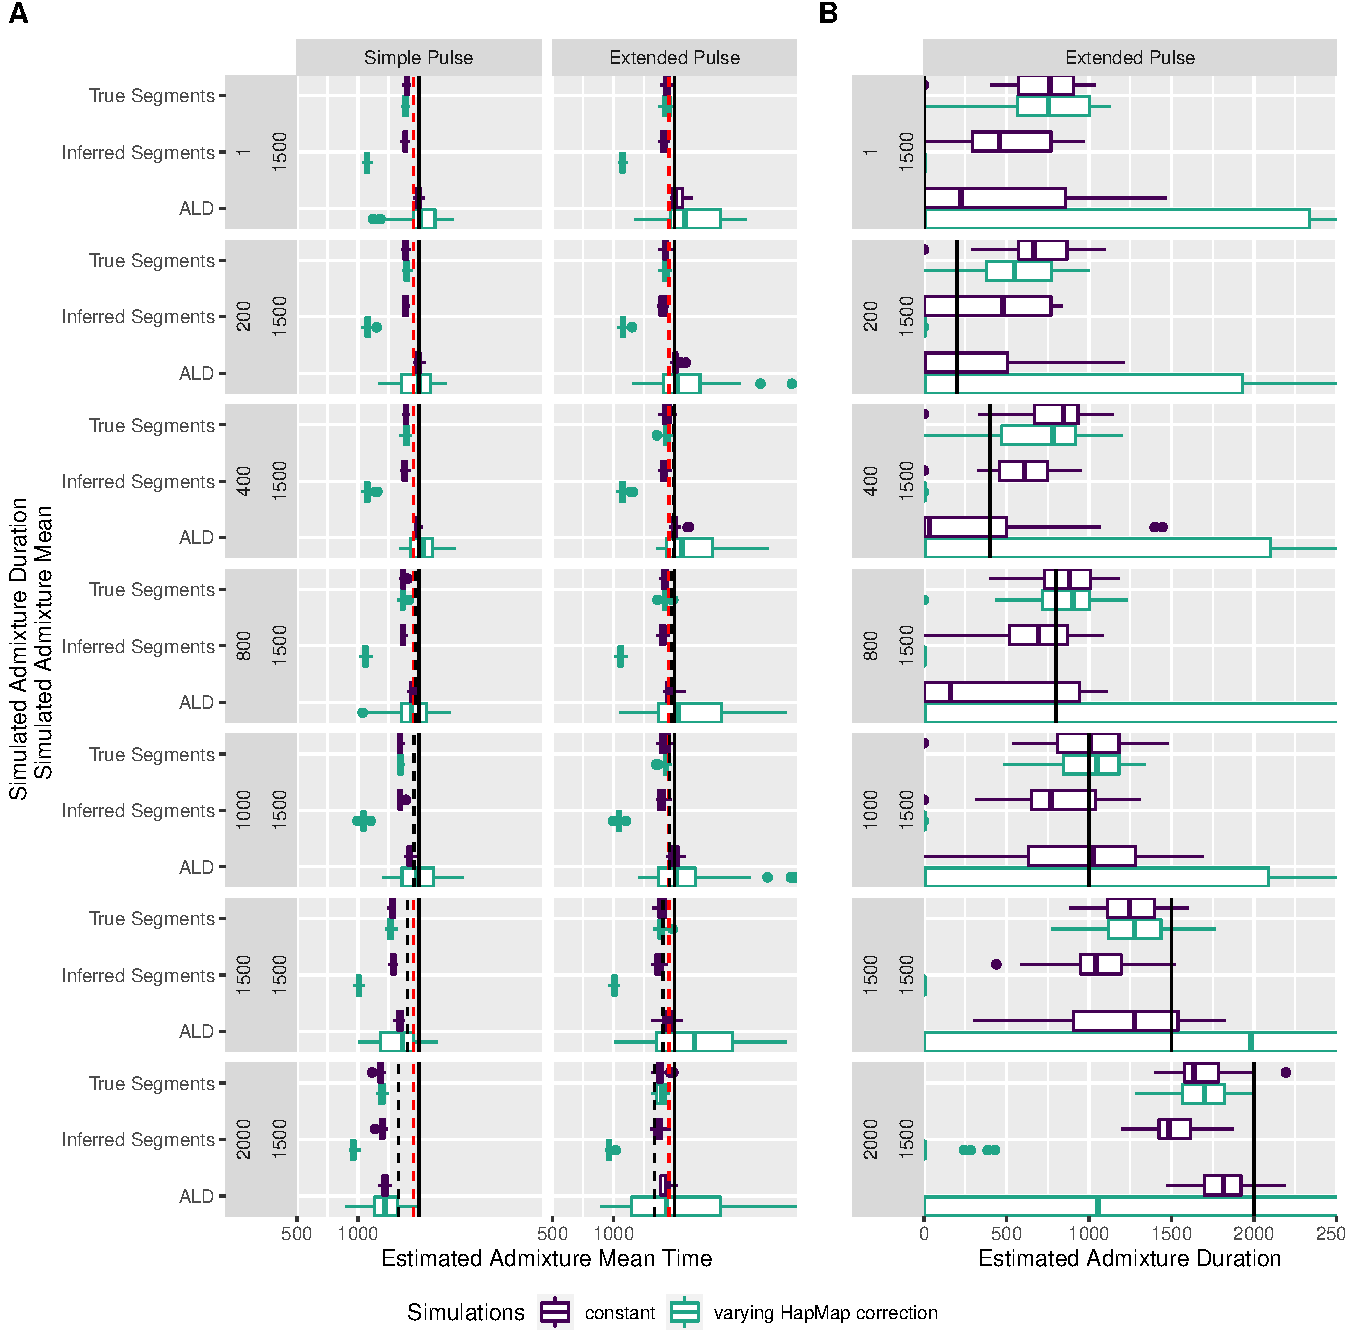
\includegraphics[width=16cm,height=18cm,keepaspectratio]{ATE_Revisions_files/figure-latex/figResult2_1-1.pdf}
\caption{\label{fig:fig3} Comparison between the simple and extended pulse one true and inferred segment length and ALD decay estimates using a constant recombination rate and an empirical recombination map for simulations with a fixed mean time ($t_m$) of 1500 generations ago and varying durations ($t_d$) . A) mean time estimates of admixture B) Extended pulse estimate for admixture duration. Solid black line indicates true $t_m$ and $t_d$, black dotted line indicates expected inverse of the mean segment length under the extended pulse model, red dotted line indicates migration corrected admixture time ($t_m$(1-m)) }
\end{figure}

\begin{figure}
\centering
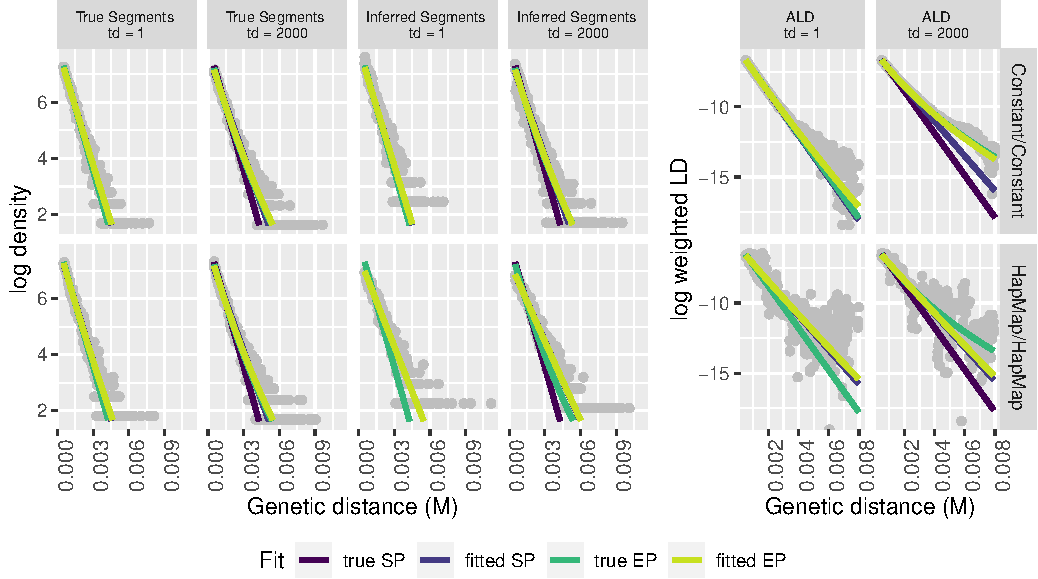
\includegraphics[width=16cm,height=18cm,keepaspectratio]{ATE_Revisions_files/figure-latex/figResult2_2-1.pdf}
\caption{\label{fig:fig3_2} Comparison of the fit to data between the simple and extended pulse using true and estimated parameters. }
\end{figure}

\begin{figure}
\centering
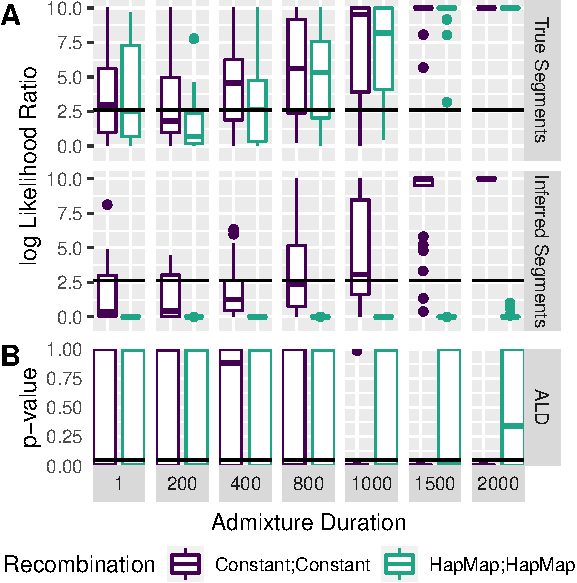
\includegraphics[width=8cm,height=9cm,keepaspectratio]{ATE_Revisions_files/figure-latex/figResult2_3-1.pdf}
\caption{\label{fig:fig3_3} Comparison of the fit to data between the simple and extended pulse using true and estimated parameters. }
\end{figure}

\subsection{Comparing effect sizes for technical covariates}\label{comparing effect sizes}

As the effect of ongoing gene flow is relatively minor, we next evaluate its relative importance for inference compared to other common assumptions made in the inference of admixture times. 

We contrast the effect of extended gene flow on admixture time inference with  the effects of a complex demographic history (Supplement Figure \ref{fig:figS1}B) and a variable recombination map (\emph{i.e.} using an empirical map for simulations but assuming a constant rate for the analysis), as well as the impact of the ascertainment scheme used to amplify Neandertal introgressed variants in the analysis, the minimum genetic distance between variants ,$d_0$, in the ALD estimation and the accuracy of the ALD estimates using a simple and complex setting for each of these parameters. 

In Figure \ref{fig:fig3}, we present the effect sizes of these four predictors on the admixture time inference. These effect sizes are estimated using a GLM on simulations under all possible parameter combinations  (S. \ref{fig:figS2_1}, Supplement Table \ref{tab:tableS1}).

As a baseline, for comparison, we define a standard model as one using the lower-enrichment ascertainment scheme (LES), $d_{0}$ = 0.05 cM, all SNPs used for ALD estimation, simple demography and constant recombination rate over the chromosome. 

As shown in the previous section, under the standard model admixture times are well-estimated, with a mean standardized difference of  -0.03 (-0.07 - 0.02 $C.I._{95\%}$) from the true
admixture time.

We find that the  inclusion of a variable recombination map leads to a large underestimate of admixture times -0.67 -0.71 -- -0.32 $C.I._{95\%}$. In contrast, all other covariates had relatively moderate effect sizes. The extended pulse   (-0.13,  -0.18 -- -0.08) is in the range of biases arising from the ascertainment scheme (-0.10, -0.16 --
-0.04), a more complex demography (-0.12, -0.16 -- -0.07) and the upward bias caused by a different $d_0$ (0.14, 0.09 --
0.18) (S. Figure \ref{fig:figS2}). The use of only 5 \% of the available SNPs for ALD estimation did not show an significant effect (0.03, -0.02 -- 0.07). We neither found a significant effect of the interaction between the ascertainment scheme and number of SNPs used for ALD estimation (0.05, -0.04 -- 0.14) (S. Figure \ref{figS2_1}, S Table \ref{xx}). 

Overall the bias introduced by the ascertainment, minimal distance
cutoff, demography and admixture model are small: around +/-0.15 standard deviations or less. The major uncertainties in the admixture time
estimate arise from assuming a constant recombination rate. The
admixture time estimates for a simple or extended admixture pulse are similarly affected by the other modeling parameters.

\begin{figure}
\centering
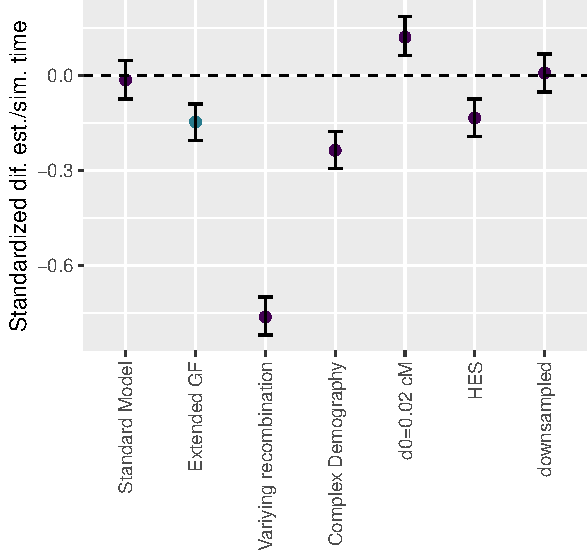
\includegraphics[width=8cm,height=16cm,keepaspectratio]{ATE_Revisions_files/figure-latex/figResult_3-1.pdf}
\caption{\label{fig:fig3} GLM effect size estimates and 95\% C.I. for the parameters: gene flow model (simple/extended), recombination rate (constant/varying), demography (simple/complex), minimal genetic distance (0.02/0.05 cM), SNPs used for ALD calculation (100 \% / 5 \%) and ascertainment scheme (LES/HES), on the standardized difference between simulated and estimated admixture time. Estimates are calculated across all possible combinations of parameters and are given as the estimate of the standard model plus the respective parameter estimate. Dotted horizontal line indicates unbiased admixture estimates.}
\end{figure}

\subsection{Application to Neandertal data}

In the previous section, we have shown using simulations that it might be difficult to distinguish admixture scenarios of various durations particularly if these happened a long time ago (i.e. more than 500 generations ago). To evaluate whether this is also true for real data, we estimated the Neandertal admixture pulse from the 1000 genomes data. We use the ALD, since it proved to be more robust compared to the direct segment inference. We fit  pulses with durations ranging from one generation up to 2,500 generations to the ALD decay curve (Figure \ref{fig:fig5}, S. Table \ref{tab:tableS2}). Plotting these best-fit ALD curves (Figure \ref{fig:fig5}A) on a y-axis in natural scale shows the extremely slight difference predicted under these drastically different gene flow scenarios. The difference between scenarios becomes more apparent if we log-transform the y-axis (Figure \ref{fig:fig5}B), where we see that ongoing gene flow results in a heavier tail in the ALD distributions. However, these LD values are very close to zero, and are thus only very noisily estimated. Therefore, we find that all scenarios are compatible with the observed data, and that there is little power to differentiate different cases. From the residual sum-of-squares and model comparison using AIC, the models perform equal, with longer extended pulses of gene flow achieving better fits (S. Table \ref{tab:tableS2_2}).




\begin{figure}
\centering
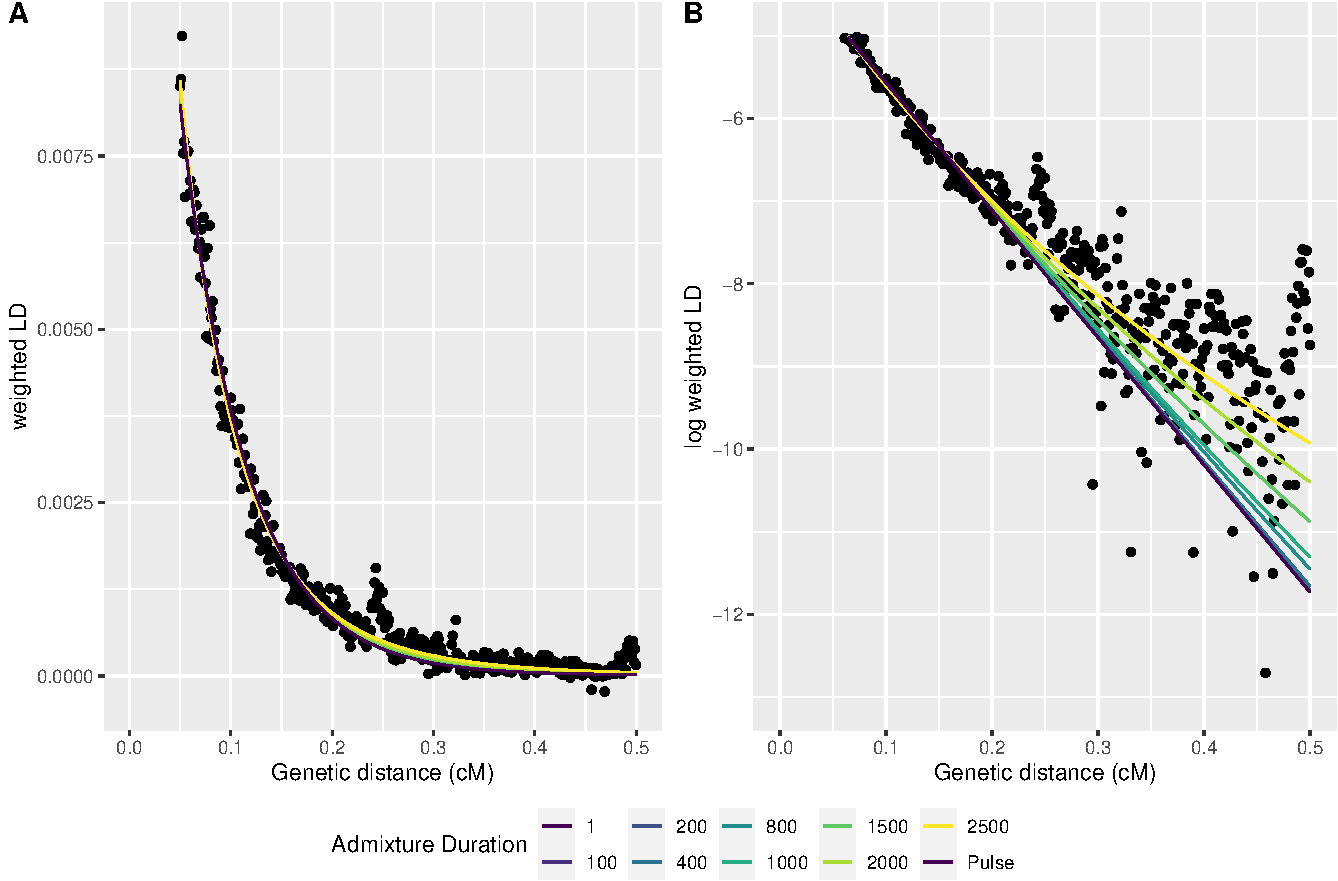
\includegraphics[width=16cm,height=18cm,keepaspectratio]{Admixture_Time_Inference_Paper_Draft_files/figure-latex/fig5-1.pdf}
\caption{\label{fig:fig5} Different admixture duration models ranging
from a one generation pulse to 2500 generations of gene flow for Neandertal interbreeding using all 1k Genome CEU individuals as the admixed population
with all YRI and 3 high coverage Neandertals as reference populations. A) Weighted LD normal scaled B) Weighted LD log scaled.}
\end{figure}

\section{Discussion}\label{discussion}
Previous estimates to date Neandertal-human gene flow have focused almost entirely on the mean time of gene flow, for which reasonably tight credible intervals can be estimated \citep{sankararaman_date_2012, moorjani_genetic_2016}. Here, we show that this simple pulse model cannot be used to establish bounds on when gene flow happened, as scenarios involving hundreds of generations of gene flow are indistinguishable from a short interval of gene flow. This means that while substantial amounts of gene flow happened around these mean times, substantial gene flow might have happened tens of thousands of years before or after these bounds. This is of great practical importance, as it might be tempting to link the genetic admixture date estimates with biogeographical events \citep{sankararaman_date_2012,lazaridis_genomic_2016,douka_age_2019,jacobs_multiple_2019,vyas_analyses_2019}. 

The discovery of early modern human genomes dated to 40,000 - 45,000 ya with very recent Neandertal ancestors less than ten generations ago \citep{fu_genome_2014, hajdinjak_early_2021} illustrates that gene flow likely happened over at least several thousand years.  In general, inference based on ancient genomes \citep{fu_genome_2014, fu_early_2015, moorjani_genetic_2016} promise to resolve some of these dating issues, as the time difference between gene flow and sampling time is much lower. However, using these genomes for dating leads to further hurdles, particularly pertaining to the spatial distribution of admixture events; whereas we can assume that the spatial structure present in initial upper paleolithic modern humans is largely homogenized in present-day people, the introgression signals observed in Bacho-Kiro and Oase could be partially private to these population, and thus these samples may have a different admixture time distribution than present-day people.

The uncertainty over the duration of Neandertal gene flow might also have some implications for selection on introgressed Neandertal haplotypes. Neandertal alleles have been suggested to be deleterious in modern human populations due to an increased mutation load \citep{harris_genetic_2016, juric_strength_2016}. Some details of these models may be slightly affected if migration occurred over a longer time. For example, \cite{harris_genetic_2016} suggested that an initial pulse of gene flow of up to 10\% Neandertal ancestry might be necessary to explain current amounts of Neandertal ancestry, with very high variance in the first few generations after gene flow. More gradual introgression could mean that such high admixture proportions were never achieved, but rather a continuous migration-selection balance process persisted for the contact period, where deleterious Neandertal alleles continually entered the modern human populations, but were selected against immediately. 
However, in terms of the overall frequencies achieved, there is likely little difference. For example, \cite{juric_strength_2016} showed using a two-locus model that the frequencies of Neandertal haplotypes alone cannot be used to distinguish different admixture histories.

In addition, we find that modelling and method assumptions have an impact on admixture time estimates that are of a similar or larger magnitude than the effect of assuming a one-generation pulse. Especially recombination rate variation may pose a practical limitation to the accuracy of admixture date estimates, and has to be very carefully considered when making inferences about admixture times. This is because both an extended pulse, as well as a non-homogeneous recombination map, lead to an admixture segment distribution that deviates from the expected exponential distribution. Correcting for just one of these factors may thus potentially conflate these issues, and can lead to a substantial underestimate of mean admixture times \citep{sankararaman_date_2012}. Therefore, population-specific fine-scale recombination maps are needed for accurate admixture time estimates, at least for admixture that happened more than a thousand generations ago. Estimates of more recent admixture appear to be somewhat more robust, perhaps because coarser-scale recombination maps are better estimated and differ less between populations \citep{hinch_landscape_2011}. 


To further refine admixture timing, time series data from more admixed early modern human and Neandertal genomes are  needed. In particular, measures based on population differentiation  \citep[e.g][]{wall_higher_2013,browning_analysis_2018,villanea_multiple_2019} are very promising to understand the different events that contributed to archaic ancestry in present-day humans. While Neandertal ancestry in present-day people has been largely homogenized due to the substantial gene flow between populations, samples from both the Neandertal and early modern human populations immediately involved with the gene flow could likely refine when and where this gene flow happened. 


\section{Material \& Methods}\label{methods}

\subsection{Power Analysis}\label{power analysis}

To test the power of distinguishing the simple from an extended pulse we simulated 100, 1000, 10000 and 100000 unique times $t$ form a Gamma distribution implemented in the R \texttt{stats v.3.6.2} package \citep{R_Core_Team_2019}, with shape parameter $k$ and scale being $k/t_m$. Where $t_m$ is 1500 generations ago. We defined $k$ for different durations as $k=1/((t_d/(4t_m))^2)$. Segment length are obtained by sampled for each $t$ from an exponential distribution (\texttt{stats v.3.6.2} package) with rate parameter $t$ for present day samples and $t_{closer}= t - t_m - t_d/2 -50$ for sampling 50 generations after the end of gene flow.
We fit the simple (\ref{xx}) and extended pulse (\ref{xx}) using the \texttt{optim} function implemented in the R \texttt{stats v.3.6.2} package. The log likelihoods are compared using a log likelihood ratio test.

\subsection{Coalescent Simulations}\label{coalescent simulations}

We test our approach with coalescence simulations using  \texttt{msprime} 
\citep{kelleher_efficient_2016}. We focus on scenarios mimicking Neandertal admixture, and choose sample sizes to reflect those available from the 1000 Genomes data \citep{the_1000_genomes_project_consortium_global_2015}. For ALD simulations we simulate 176 diploid
African individuals and 170 diploid non-Africans, corresponding to the
number of Yoruba (YRI) and Central Europeans from Utah (CEU). For segment simulations we simulated 50 diploid diploid non-Africans.
Since three high coverage Neandertal genomes are available \citep{prufer_complete_2013,prufer_high-coverage_2017,mafessoni_high_coverage_2020} we  simulate three diploid Neandertal genomes. For each individual we simulate 20
chromosomes with a length of 150 Mb each. The mutation rate is set for
all simulations to \(2*10^{-8}\) per base per generation. The
recombination rate is set to \(1*10^{-8}\) per base pair per generation
unless specified otherwise. The demographic parameters are based on
previous studies dating Neandertal admixture
\citep{sankararaman_date_2012,fu_genome_2014,moorjani_genetic_2016}. In
the ``simple'' demographic model (S. Figure  \ref{fig:figS1} A), the effective
population size is assumed constant at $N_e=10,000$ for all populations, the
split time between modern humans and Neandertals is 10,000 generations
ago and the split between Africans and non-Africans is 2,550
generations ago. The migration rate from Neandertals into non-Africans
was set to zero before the split from Africans, to ensure that there is no Neandertal
ancestry in Africans. Each simulation was repeated 100 times. For the comparison of segment and ALD data we followed the demographic model simulation setup of \cite{skov_detecting_2018}, but only simulated the Europeans. The split time of  non-Africans are kept the same as in the ALD simulations (2550 generations ago) (S. Figure \ref{fig:figS1}C).  


\subsubsection{Simulating admixture}\label{Simulating the expanded pulse}
We specify simulations under the extended pulse model using the mean admixture time $t_m$ and the duration $t_d$. We recover the simple pulse model by setting $t_d=1$. To obtain the migration rates in each generation, we use a discretized version of the migration density (eq \ref{eq:RV_extended_pulse}), which we then scale to the total amount of Neandertal ancestry in modern humans (here 0.03). 

\subsubsection{Recombination maps}\label{recombination map}
Uncertainties in the recombination map were previously shown to influence admixture time estimates \citep{sankararaman_date_2012,fu_genome_2014,sankararaman_combined_2016}. To investigate the effect of more realistic
recombination rate variation, we perform simulations using empirical recombination maps. We use the  African-American map \citep{hinch_landscape_2011} for simulations to evaluate the relative importance of simulation and modeling parameters for admixture time estimates. The HapMap phase 3 map \citep{HapMapConsortium_second_2007} is used for evaluating inference using the extended pulse model. For simplicity, we use the same
recombination map (150 Mb of chromosome 1, excluding the first 10 Mb)
for all simulated chromosomes. When simulating under an empirical map, with the analysis assuming a constant rate (\emph{i.e.} no correction), we use the mean recombination rate from the respective map to calculate the genetic distance from the physical distance for each SNP. The mean recombination rate is
calculated from the 150 Mb map (\(1.017 \, \frac{cM}{Mb}\) AAMap,
\(0.992 \, \frac{cM}{Mb}\) HapMap.



\subsubsection{Complex demography}\label{inferred demography}
Demographic factors such as population size changes are known to influence LD
patterns, and may thus influence admixture time estimates \citep{gravel_population_2012,liang_lengths_2014}. To test the impact of
demographic history on admixture time estimates, we contrast our standard model with a more 
realistic and complex demographic history(S. Figure \ref{fig:figS1} B). The effective population
sizes change over time, are based on estimates from Neandertal and present-day human genomes. In particular, we use the MSMC estimates for YRI and CEU to model Africans and Europeans, respectively 
\citep{schiffels_inferring_2014}. The Neandertal population size history is modelled after  PSMC estimates \citep{li_inference_2011} using the high-coverage Vindija 33.19 genome
\citep{prufer_high-coverage_2017}. 

The split times between Neandertals and
modern humans is kept the
same as in the simple demographic simulations (10,000 generations ago) (S. Figure  \ref{fig:figS1} A). We add substructure within Africa starting from 3,200 till 2,550 generations ago with a per generation migration rate between the two subpopulations of 0.001. The population size of the common ancestor of Neandertals and humans  is set to 18,296 (based on MSMC results). To mimic the age of the samples, Neandertals are sampled 750 generations before the Africans and non-Africans. Finally, we add recent gene flow between African and non-African populations with a total migration rate of 0.01 starting from 200 till 50 generations ago \citep{petr_limits_2019}.



\subsection{Ascertainment scheme}\label{asceteinment scheme}
Since ALD for ancient admixture events can be quite similar to the genomic background, SNPs need to be ascertained to enrich for
Neandertal informative sites in the test population.This removes noise and
amplifies the ALD signal \citep{sankararaman_date_2012}. 
We evaluate the impact of the ascertainment scheme by contrasting two distinct schemes \citep{sankararaman_date_2012,fu_genome_2014}. The lower-enrichment ascertainment scheme (LES) only considers  sites that are fixed for the ancestral state in
Africans and polymorphic or fixed derived in Neandertals. The higher-enrichment
ascertainment scheme (HES) is more restrictive in that it further excludes all sites that are not polymorphic in non-Africans.

\subsection{ALD calculation}\label{ALD calculation}

The pairwise weighted LD between the ascertained SNPs a certain genetic
distance \(d\) apart is calculated using ALDER
\citep{loh_inferring_2013}. A minimal genetic distance \(d_0\) between
SNPs is set either to 0.02 cM and 0.05 cM. This minimal distance cutoff
removes extremely short-range LD, which might also be due to inheritance of segments from the ancestral population (incomplete lineage sorting ILS) and not gene flow. 




\subsection{Modeling parameter effect sizes}\label{modeling prameter effect sizes}

We consider a set of five parameters:
\begin{itemize} 
    \item ascertainment scheme: $A_i$ = LES/HES
    \item minimal genetic distance: $M_i$ = $0.02 cM/ 0.05 cM$
    \item demography: $D_i$ = simple/complex
    \item recombination rate: $R_i$ = constant/variable
    \item n SNPs used: $G_i$ = 100 \%/5 \%
    \item gene flow model: $G_i$ = simple/extended
\end{itemize}

We perform simulations using all possible parameter combinations. For the effect of the amount of SNPs i.e. accuracy of the ALD estimates, we downsampled the data by randomly choosing 5 \% of the overall SNPs for ALD calculation.
We define a standard model having a constant recombination rate, simple demography and gene flow, LES ascertainment and $d_0 = 0.05$.
The genetic distance is assigned from the physical  position using the average recombination rate of the African-American genetic map (\emph{i.e.}, assuming the recombination rate is constant over the simulated chromosome given by this value) for simulations under a variable recombination rate.
For each of the possible sets of parameters, we simulate 100 replicates each and fit ALD decay curves. We excluded a very small number of simulations for which the curve could not be estimated (66 out of 6,400). 



To estimate the effect size of the different parameters (eq.
\ref{eq:GLM1}) we use a Bayesian Generalized Linear Model (GLM):

\begin{equation}\label{eq:GLM1}
\begin{split}
E_i &\sim \text{Normal}(\mu_i,\sigma) \\
\mu_i &= \alpha + \beta_aA_i + \beta_mM_i + \beta_dD_i + \beta_rR_i + \beta_{s}S_i + \beta_gG_i \\
\alpha &\sim \text{Normal}(0,2) \\
\beta_a,\beta_m,\beta_d,\beta_r,\beta_{s},\beta_g &\sim \text{Normal}(0,2) \\
\sigma &\sim \text{Exponential}(1)
\end{split}
\end{equation}

\begin{equation}\label{eq:GLM2}
\begin{split}
E_i &\sim \text{Normal}(\mu_i,\sigma) \\
\mu_i &= \alpha + \beta_aA_i + \beta_mM_i + \beta_dD_i + \beta_rR_i + \beta_{s}S_i + \beta_gG_i + \beta_{as}S_i A_i\\
\alpha &\sim \text{Normal}(0,2) \\
\beta_a,\beta_m,\beta_d,\beta_r,\beta_{s},\beta_g &\sim \text{Normal}(0,2) \\
\sigma &\sim \text{Exponential}(1)
\end{split}
\end{equation}

The response variable $E_i$ for this model are the residuals, \emph{i.e.}, the difference between the estimated admixture time $t_{est}$ and simulated admixture time $t_{sim}$ for each simulation:
$$E_i = \frac{t_{est} - t_{sim}}{\sigma_{t_{est}}}$$, where $\sigma$ is the standard deviation of $t_{est}$ , and the model variables $A, M, D, R, S$ and $G$ are binary predictors. We also modeled the interaction between number of used SNPs and the ascertainment scheme using the GLM described in \ref{eq:GLM2} with an additional predictor for the interaction $as$.
We assume a Normal likelihood because it is the maximum entropy distribution in our case. We obtained the posterior probability using a Hamiltonian Monte Carlo MCMC algorithm, as implemented in STAN \citep{carpenter_stan_2017} using an R interface \citep{stan_development_team_rstan_2018,mcelreath_statistical_2020}. The Markov chains converged to the target distribution (Rhat = 1) and efficiently sampled from the posterior (S. Table \ref{tab:tableS1}).  

\subsection{Estimating admixture time from simulated segment data}\label{Estimating admixture time from simulated segment data}

For estimating admixture time and duration from introgressed segments, we used the true segment length obtained from \texttt{msprime} or inferred the segments using the HMM from \cite{skov_detecting_2018}. We only considered inferred segments with a posterior decoding of 0.9 or higher. Furthermore, we use an upper and lower cutoff for inferred segment length of 0.05 cM and 1.2 cM. The genetic length are assigned using the true constant recombination rate for segments simulated under a constant rate. For simulations under an empirical map (HapMap map) we either used the mean recombination rate of the HapMap, the AAMap or the HapMap.
We fit the simple (\ref{xx}) and extended pulse (\ref{xx}) using the \texttt{optim} function implemented in the R \texttt{stats v.3.6.2} package (method="L-BFGS-B") with lower and upper constrains being $1/5000$ for $t_m$ and $2/1e8$ for $k$. The log likelihoods for the two fits are compared using a log likelihood ratio test.

\subsection{Estimating admixture time from real data}\label{Estimating admixture time from real data}
To evaluate when we can reject a given admixture durations (including a one generation pulse), we applied the extended pulse model on real data from the 1000 Genomes project \citep{the_1000_genomes_project_consortium_global_2015}.

We used the 1000 Genomes phase 3 data together with the Altai, Vindija and Chagyrskaya high coverage Neandertals, including the 107 unrelated individuals from the YRI as representatives of unadmixed Africans and all CEU as admixed Europeans. We only consider biallelic sites, and determine the ancestral allele using  the Chimpanzee reference genome (panTro4). We used the CEU specific fine-scale recombination map \citep{spence_inference_2019} to convert the physical distance between sites into genetic distance. 


\section{Acknowledgments}

We thank Svante P\"a\"abo, Janet Kelso, Fabrizio Mafessoni, St\'{e}phane Peyr\'{e}gne, Laurits Skov, Divyaratan Popli, Alba Bossom Mesa and Arev S\"umer for helpful comments and discussions.
This work was supported by the Max Planck Society and the European Research Council (grant number: 694707) to Svante P\"a\"abo.

\section{Data Availability}\label{Data Availability}

The simulation script, the analysis pipeline and the \emph{Extended Admixture Pulse} model is  available  on  GitHub: \url{https://github.com/LeonardoIasi/Extended_Admixture_Pulse}. No new data were generated for this study.

\section{Competing interests}

The authors declare that they have no competing interests.

\hypertarget{refs}{}

\bibliography{References/MyLibraryATE}


%\pagebreak
%\setcounter{figure}{0} %\renewcommand{\figurename}{Fig. S}
%\renewcommand{\tablename}{Tab. S}




\end{document}